Implementeringen af sht21p er sket ved at designe et print som indeholder sht21p og et 2. ordensfilter. 
Da sht21p-komponentet er et SMD-komponent var det ikke muligt at opstille kredsløbet på vero-board. Det var derfor nødvendigt at få et print produceret. Til design af printet blev CadSoft EAGLE PCB design software brugt. Nedenfor ses diagram og PCB layout af printet.


\begin{figure}[htb]
\centering
{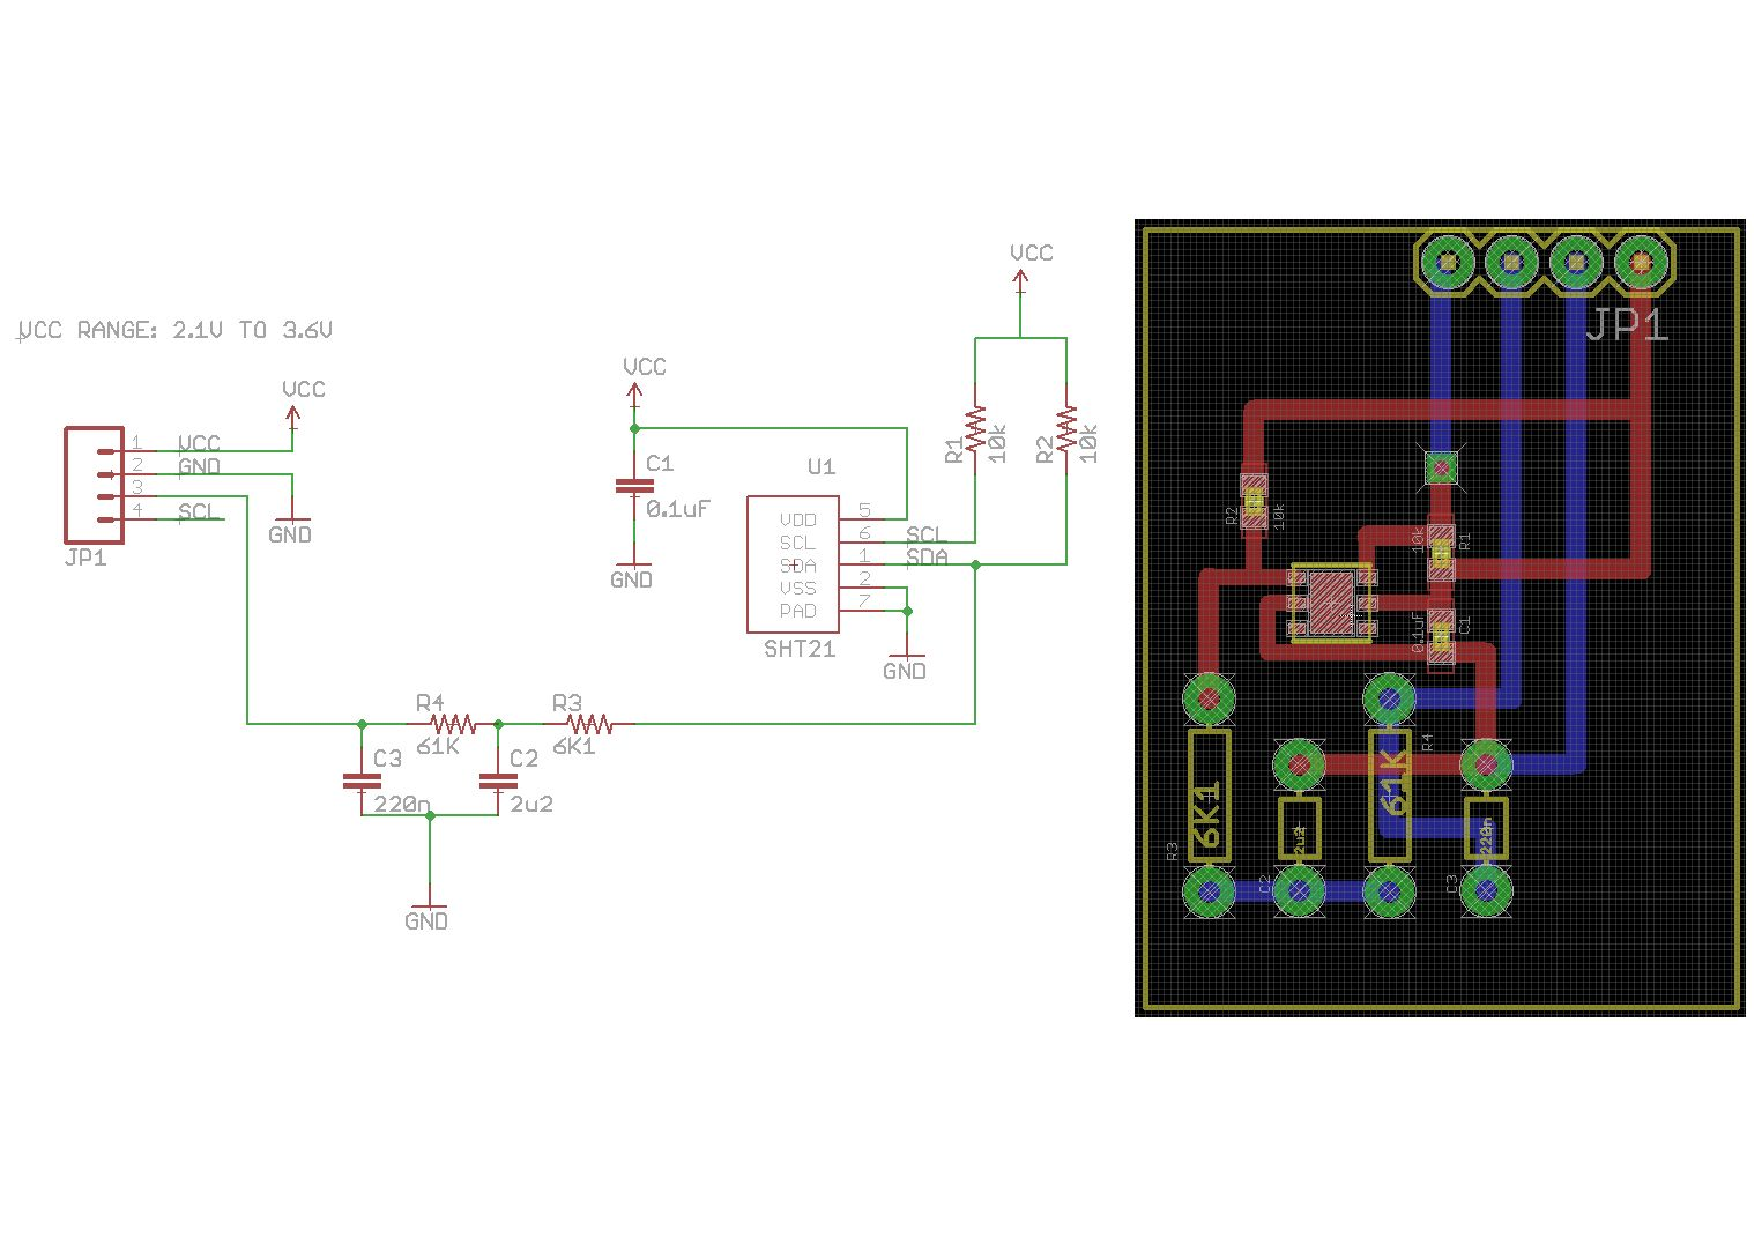
\includegraphics[width=\textwidth]{filer/implementering/SHT21P-pcb-sch}}
\caption{Schematic og layout af SHT21P kredsl\o{}b}
\label{lab:SHT21P-kredsloeb}
\end{figure}

Kredsløbet på figur \ref{lab:SHT21P-kredsloeb} blev eksporteret til gerberfiler og sendt til elektronikværkstedet som så ætsede printet og derefter monteret op.

